The Deployment Diagram shown below describes how the logical components designed in the context of the Component Diagram are to be physically deployed on the different devices needed for the functioning of the system.

As shown, the app server hosts the main logic components and manages their interaction. It provides access to them through the APIs defined in section \autoref{sec:components_interfaces} and guarantees they can access the data layer residing on the database server.
Every client with a significant application layer implements a limited subset of components responsible to interpret the inputs from the users and perform requests to the app server. When needed, an apposite module for the localization is provided as well.
The web server provides static web pages and the logic necessary to the browser to interact with the app server.

\begin{sidewaysfigure}
	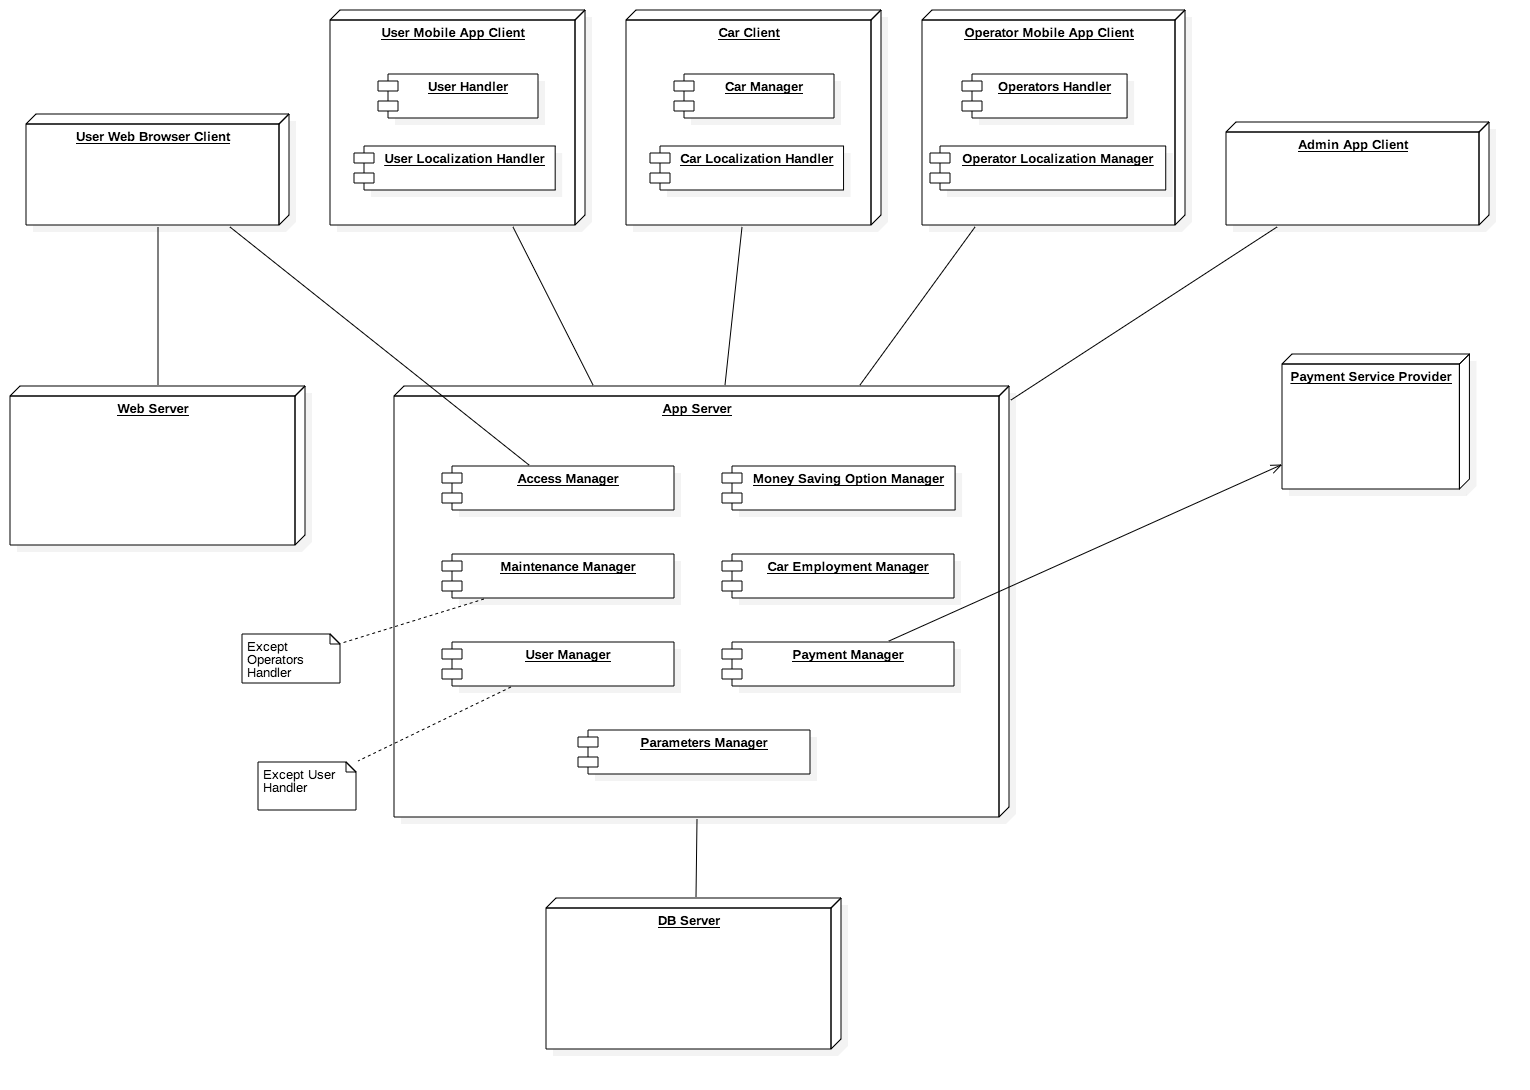
\includegraphics[width=\hsize, center]{img/deployment_diagrams/global.png}
\end{sidewaysfigure}

	\subsubsection{Non functional requirements}
		The architectural structure proposed addresses the requirements of \textit{integrity} and \textit{confidentiality} introducing a DMZ which separates with a firewall the app server, accessible from the outside network, from the database server. To avoid intrusions on the app server, another firewall is provided, with less restricting rules to allow outside clients to access. This way, even if an attack is performed to the app server, a more impenetrable layer of security still divide the intruders from the sensitive data. The structure just described is a standard pattern in the design of three-layer architectures.
		
		% TODO need to add distribution to app and db for Robustness and Performance. Also dDoS protection this way.
		
		% TODO flexibility guaranteed by the design of atomic components and stuffs.
\FloatBarrier

% TODO talk about technological choices for APIs, app server, db server, mobile apps, desktop apps, browser, ...